\documentclass[final]{article}
\usepackage[numbers,sort&compress]{natbib} % formato de citas
\usepackage{neurips}            % estilo de la conferencia NeurIPS
\usepackage[T1]{fontenc}        % letras acentuadas y comillas « » con sus propios caracteres
\usepackage[spanish]{babel}     % definiciones para el español
\usepackage{graphicx}           % para insertar figuras
\usepackage{amsmath,amssymb}    % más símbolos útiles
\usepackage[hidelinks]{hyperref}% para los links
\usepackage{multirow}           % algunas mejoras para las tablas
\usepackage{booktabs}
\usepackage{endnotes}           % las citas textuales van todas juntas al final
\let\footnote=\endnote          % cada \footnote pasa a ser una nota al final
\renewcommand{\notesname}{Citas textuales}

\begin{document}
\def\tablename{Tabla}          % (sino les pone Cuadro)

\title{Conducción autónoma en calles de Santa Fe\\
       mediante neuroevolución}

\author{M. Bertona, A. Greminger y A. Nanzer \\
        Facultad de Ingeniería y Ciencias Hídricas,
        Universidad Nacional del Litoral}

\maketitle

% =====================================================================
\begin{abstract}
Enseñar a un auto a seguir una ruta urbana exige decidir el volante y el acelerador en cada instante.
Para esa tarea no hay una respuesta correcta paso a paso, y por eso no sirve entrenar con el gradiente del error.
En este trabajo, un algoritmo genético entrena una red neuronal pequeña para manejar por calles reales de Santa Fe, sin ejemplos de manejo.
El auto se simula con un modelo cinemático de bicicleta, al que se agregó un límite de agarre.
La red recibe solo información medida desde el propio auto.
Se entrena por etapas, desde una manzana hasta un recorte de tres por tres manzanas.
Se comparan cuatro operadores de cruce, dos de mutación y el efecto del límite de agarre.
Todas las redes llegan a destino en 15 a 20 de 20 rutas del centro.
También manejan en barrios que no usaron para entrenar.
Sin el límite, la red dobla las esquinas a la velocidad máxima, con aceleraciones imposibles para un auto real.
Con el límite, maneja despacio y dentro de lo físicamente posible.
La red aprende lo que la física y la función de aptitud le piden, y eso permite guiar su comportamiento.
\end{abstract}

% =====================================================================
\section{Introducción}

La conducción autónoma es uno de los problemas de control más estudiados de los últimos años.
Un auto tiene que llegar a destino, mantenerse en la calzada y respetar su carril.
Las soluciones clásicas separan el problema: un planificador elige el camino y un controlador lo sigue.
El controlador suele diseñarse con un modelo del vehículo, por ejemplo con control predictivo \cite[p.~1097]{kong2015}\footnote{Las citas textuales de estas notas son traducciones propias. «En cada instante de muestreo, $t_s = 100$\,ms, el controlador [predictivo] resuelve [un problema de optimización con el modelo del vehículo]».}.
Otra opción es aprender el controlador a partir de la experiencia, sin programar sus reglas.

Aprender a manejar tiene una dificultad: no hay un volante correcto en cada instante.
Además, la nota de un viaje cambia a saltos, por ejemplo cuando el auto choca.
Por eso la retropropagación, que necesita la salida deseada y una función derivable, no se aplica de forma directa \cite[p.~763]{montana1989}, \cite[p.~1425]{yao1999}\footnote{Montana y Davis: «Calcular un gradiente requiere que la función sea derivable. Por lo tanto, la retropropagación no puede manejar criterios de optimización discontinuos». Yao: «la función de aptitud (o de error) no necesita ser derivable, ni siquiera continua, ya que los algoritmos evolutivos no dependen de información del gradiente».}.
La neuroevolución resuelve esto: busca los pesos de la red con un algoritmo genético que solo compara viajes \cite[p.~762]{montana1989}, \cite[p.~1439]{yao1999}\footnote{Montana y Davis, sobre el problema de clasificación que estudiaron: «No solo cumple su tarea, sino que supera a la retropropagación». Yao recomienda este camino «especialmente cuando la información del gradiente de la función de error es difícil o costosa de obtener».}.

Togelius y Lucas la aplicaron a autos de carrera simulados, y mostraron que la red debe recibir información medida desde el propio auto \cite[pp.~1906 y 1912]{togelius2005}\footnote{«El único controlador capaz de evolucionar un buen comportamiento de carrera fue el basado en una red neuronal que actúa sobre entradas egocéntricas».}.
En otro trabajo lograron controladores generales al pasar de pistas simples a pistas complejas \cite[p.~1194]{togelius2006}\footnote{«Esto se puede lograr con evolución incremental, yendo de pistas más simples a más complejas [\dots]. Los intentos de evolucionar controladores generales con la mutación de sensores activada fallaron, como también los intentos de evolucionar controladores en todas las pistas a la vez».}.
Gomez y Miikkulainen llegaron a lo mismo: una tarea que no se aprende directo sí se aprende de a poco \cite[p.~11]{gomez1996}\footnote{«Este trabajo muestra que, aun cuando una tarea es demasiado difícil para evolucionarla directamente, la neuroevolución puede aplicarse de forma incremental para lograr el comportamiento complejo buscado».}.
Por último, Nelson y colaboradores señalan que la función de aptitud decide qué comportamiento aparece \cite[p.~365]{nelson2009}\footnote{«La función de aptitud gobierna: (1) las propiedades funcionales de los controladores evolucionados; (2) el punto en que el entrenamiento se estanca por falta de señal de aptitud; y (3) el grado en que se aprende un comportamiento nuevo».}.

Los trabajos de Togelius y Lucas usan pistas cerradas, sin carriles y sin cruces de calles.
En una ciudad, en cambio, el auto tiene que doblar a ambos lados y mantenerse en su mano.
Además, el modelo cinemático no limita el agarre de las ruedas, y deja doblar a cualquier velocidad \cite[p.~1098]{kong2015}\footnote{«Incluso un controlador bien ajustado puede tener problemas para seguir una trayectoria con alta aceleración lateral, porque la diferencia con el modelo se vuelve más marcada».}.
Una red entrenada sobre ese modelo puede aprovechar esa falla en lugar de aprender a manejar.
Los mismos autores proponen limitar la velocidad para que la aceleración lateral no supere cierto valor \cite[p.~1099]{kong2015}\footnote{«Para mejorar el desempeño, el planificador de trayectorias también puede limitar la velocidad de referencia, de modo que la aceleración lateral no pueda superar cierto valor».}.

En este trabajo, un algoritmo genético entrena un perceptrón multicapa para manejar por calles reales de Santa Fe.
Un planificador clásico elige las calles, y la red solo decide el volante y el acelerador.
Al modelo del auto se le agrega un límite de aceleración lateral: para tomar una esquina hay que llegar despacio.
La red se entrena por etapas, y se comparan operadores que tratan a cada neurona como una unidad con otros que tratan cada peso por separado.
% =====================================================================
\section{Neuroevolución de un controlador de manejo}
\label{sec:metodos}

El sistema une un planificador clásico con una red que maneja.
El mapa de calles es un grafo, y el algoritmo A* elige el camino más corto \cite{hart1968}.
En cada paso, los sensores alimentan a la red, que decide el volante y el acelerador.
Al final del viaje, una función de aptitud califica a la red, y el algoritmo genético forma con esas notas la población siguiente.

% ---------------------------------------------------------------------
\subsection{Mapas, rutas y vehículo}

Las calles se descargan de OpenStreetMap con OSMnx \cite{boeing2025}.
Cada calle tiene dos manos de 3,5\,m.
Para entrenar se usan una manzana, donde el auto da vueltas, y recortes de 2$\times$2 y 3$\times$3 manzanas del centro (Fig.~\ref{fig:mapas}).
Para probar se usan el centro completo y seis barrios.
El camino de cada viaje se corre 1,75\,m a la derecha, al centro del carril.
Sobre esa línea hay un punto de control cada 10\,m y otro en cada giro de 30$^\circ$ o más.
Un punto se alcanza a menos de 6\,m, y los puntos solo cuentan en orden \cite[p.~1190]{togelius2006}\footnote{«Los puntos solo se pueden pasar en el orden correcto, y un punto cuenta como pasado cuando el centro del auto está a menos de 30 píxeles de él».}.
Si el auto se abre en un giro y alcanza uno de los dos puntos siguientes, los salteados también cuentan.

\begin{figure}[!htb]
\centering
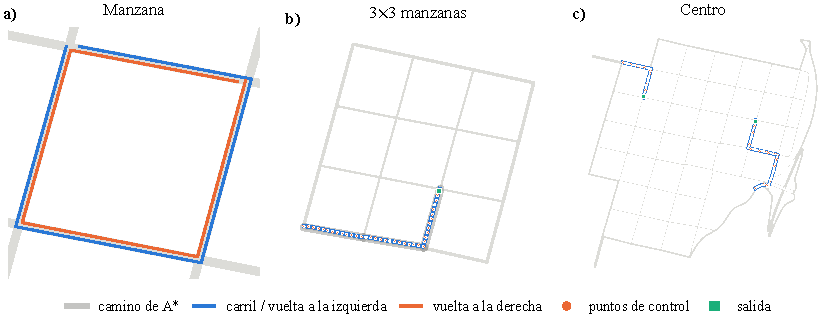
\includegraphics[width=0.7\linewidth]{figuras/fig_mapas.pdf}
\caption{Mapas de calles reales de Santa Fe. a) Manzana de la primera etapa, con una vuelta hacia cada lado. b) Recorte de 3$\times$3 manzanas con una ruta: el camino de A*, el carril derecho y los puntos de control. c) Centro de la ciudad con dos rutas al azar.}
\label{fig:mapas}
\end{figure}

El auto se simula con el modelo cinemático de bicicleta \cite[p.~1095]{kong2015}\footnote{«Las entradas de control son los ángulos de dirección delantero y trasero y la aceleración. Como en la mayoría de los vehículos las ruedas traseras no giran, suponemos $\delta_r = 0$».}.
Su estado es $(x, y, \psi, v)$ y sus entradas son el volante $\delta$ y la aceleración $a$:
\begin{equation}
  \dot x = v\cos(\psi+\beta), \quad
  \dot y = v\sin(\psi+\beta), \quad
  \dot \psi = \frac{v}{\ell_r}\sin\beta, \quad
  \dot v = a, \quad
  \beta = \arctan\!\left(\frac{\ell_r}{\ell_f+\ell_r}\tan\delta\right),
  \label{eq:bicicleta}
\end{equation}
con $\ell_f = 1{,}1$\,m y $\ell_r = 1{,}7$\,m \cite[p.~1095]{kong2015}\footnote{«El vehículo de prueba fue un Hyundai Azera (distancia entre ejes de 2,843\,m, $\ell_f = 1{,}105$\,m y $\ell_r = 1{,}738$\,m)». Aquí se usan esos valores redondeados.}.
Se integra con el método de Euler cada 0,1\,s \cite[p.~1095]{kong2015}\footnote{«Los modelos se discretizan con el método de Euler y se muestrean cada 100\,ms o cada 200\,ms».}.
El volante se limita a $\pm35^\circ$, la aceleración a entre $-4$ y $+2$\,m/s$^2$ y la velocidad a 11\,m/s.
El viaje termina si alguna esquina del auto, de 4,5\,m por 1,8\,m, sale de la calzada.

\begin{figure}[!htb]
\centering
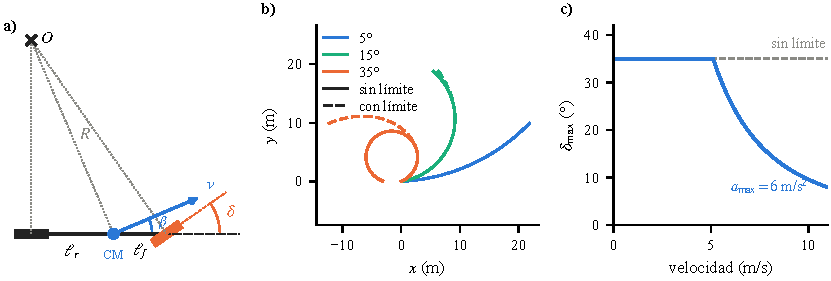
\includegraphics[width=0.7\linewidth]{figuras/fig_auto.pdf}
\caption{Modelo del vehículo. a) Modelo de bicicleta: CM es el centro de masa y $O$ el centro de giro. b) Trayectorias de 5\,s con el volante fijo y el acelerador a fondo, sin límite de agarre (continuo) y con límite de 6\,m/s$^2$ (discontinuo). c) Volante máximo permitido en función de la velocidad, según \eqref{eq:agarre}.}
\label{fig:auto}
\end{figure}

Para que el auto no doble a fondo a cualquier velocidad, se limita el volante: la aceleración lateral $a_y = v^2\sin\beta/\ell_r$ no puede superar $a_{\max} = 6$\,m/s$^2$.
De ahí sale el volante máximo a cada velocidad,
\begin{equation}
  \delta_{\max}(v) = \min\!\left(35^\circ,\ \arctan\!\left(\frac{\ell_f+\ell_r}{\ell_r}\tan\beta_{\max}\right)\right),
  \qquad \sin\beta_{\max} = \frac{a_{\max}\,\ell_r}{v^2}.
  \label{eq:agarre}
\end{equation}
Por debajo de 5,1\,m/s se puede doblar a fondo, pero a 8\,m/s el volante queda limitado a 14,9$^\circ$ (Fig.~\ref{fig:auto}c).
El límite no frena al auto: si la red llega rápido a una esquina, se sale, así que tiene que aprender a llegar despacio.

% ---------------------------------------------------------------------
\subsection{Red, aptitud y operadores genéticos}

La red recibe 16 entradas, todas medidas desde el auto: siete rayos hasta el borde, la velocidad, la dirección y la distancia al próximo punto, el desvío del carril y la dirección del carril 3\,m y 6\,m adelante.
Al entrenar se suma a cada entrada un ruido gaussiano de desvío 0,02 \cite[p.~1189]{togelius2006}\footnote{«Se aplica una pequeña cantidad de ruido a todas las lecturas de los sensores». El valor de 0,02 es una elección propia.}.
La red es un perceptrón $16\to16\to2$ con tangente hiperbólica: una salida es el volante y la otra el acelerador, que frena si es negativa.
Sus 306 pesos y umbrales forman el cromosoma, con un gen real por peso \cite[p.~764]{montana1989}\footnote{«Los pesos (y umbrales) de la red neuronal se codifican como una lista de números reales».}.

La aptitud de un viaje por la ruta $r$ mide el avance y castiga el tiempo fuera del carril:
\begin{equation}
  F_r = (1-\lambda)\,\frac{k_r + p_r}{K_r}\,\bigl(1 - c\,f_r\bigr) + \lambda\,L_r\left(1 - \frac{t_r}{t_{\max,r}}\right).
  \label{eq:aptitud}
\end{equation}
Aquí $k_r$ son los puntos pasados, $p_r$ el avance hacia el siguiente \cite[p.~1190]{togelius2006}\footnote{«más un término intermedio que representa cuánto avanzó hacia el siguiente punto, calculado a partir de las distancias relativas entre el auto y los puntos anterior y siguiente».}, $K_r$ el total de puntos y $f_r$ la fracción del tiempo fuera del carril.
$L_r$ vale 1 si el auto llegó, $t_r$ es la duración del viaje y $t_{\max,r}$ es el largo de la ruta dividido 4\,m/s, más 10\,s.
El avance parcial distingue a las redes aunque ninguna llegue \cite[pp.~350--351]{nelson2009}\footnote{«Si todos los controladores de la población inicial están por debajo de una competencia mínima para la función de aptitud, esta no genera presión de selección y la población no logra evolucionar».}.
Con $c=0{,}8$, ir por la mano contraria vale más que quedarse quieto.
La nota de una red es el promedio de $F_r$ en las rutas que manejó.

El algoritmo genético usa reemplazo generacional, torneo de 3 y elitismo de 2 \cite[p.~1908]{togelius2005}\footnote{«El operador de mutación se aplicó a todos los individuos, salvo a los dos más aptos». El torneo de 3 es una elección propia.}.
Dos neuronas ocultas intercambiadas dan la misma red con otro cromosoma: es el problema de las permutaciones \cite[p.~1426]{yao1999}\footnote{«Uno de los problemas del entrenamiento evolutivo de redes neuronales es el problema de las permutaciones [\dots], también conocido como problema de las convenciones en competencia».}.
Además, un cruce que separa los pesos de una neurona puede romperla \cite[p.~765]{montana1989}\footnote{«Esta sinergia es mayor entre los pesos de las conexiones que entran a un mismo nodo. Por lo tanto, al transmitirse el material genético, estos subgrupos lógicos deberían mantenerse juntos».}.
Por eso se comparan cuatro cruces: \emph{por neurona}, que copia cada neurona entera de un padre; \emph{por pesos}, que copia cada peso de un padre al azar \cite[p.~765]{montana1989}\footnote{«Este operador asigna un valor a cada posición del cromosoma del hijo eligiendo al azar uno de los dos padres y usando el valor de la misma posición en el cromosoma de ese padre».}; BLX-$\alpha$, con $\alpha=0{,}5$ \cite{eshelman1993}; y sin cruce.
También se comparan dos mutaciones: la \emph{gaussiana} suma a cada gen, con probabilidad 0,05, un ruido normal de desvío $\sigma$ \cite[p.~1427]{yao1999}\footnote{«En estos ejemplos, el principal operador de búsqueda fue la mutación gaussiana».}, y la \emph{mutación por neurona} suma ese ruido a todos los pesos de dos neuronas \cite[p.~766]{montana1989}\footnote{«Como se predijo, hay un orden claro en cuanto a rendimiento: 1) MUTATE-NODES [\dots]», que es la mutación por neurona.}.

% ---------------------------------------------------------------------
\subsection{Entrenamiento por etapas}

La población empieza dando vueltas a una manzana y pasa a mapas cada vez más grandes.
Gomez y Miikkulainen arman una población nueva en cada tarea \cite[pp.~6--7]{gomez1996}; aquí, en cambio, la población sigue de una etapa a la otra.
El desvío $\sigma_e$ de la mutación baja en cada etapa, para afinar sin desarmar lo aprendido.
Se pasa de etapa cuando la mejor red llega en una fracción $u_e$ de las rutas de referencia, tras al menos $g_{\min}$ generaciones, o cuando se agotan las $g_{\max,e}$.
La última etapa usa todas sus generaciones.

En cada generación, toda la población maneja las mismas rutas al azar.
En la manzana son 2 vueltas, una hacia cada lado; en los otros mapas, 3 rutas más 1 de una etapa anterior, para no olvidarla.
Como la nota en pocas rutas tiene ruido, la red de mayor nota maneja además rutas de referencia fijas: 8 vueltas en la manzana y 20 rutas en los otros mapas.
Reemplaza a la mejor guardada solo si llega en más de ellas, y esta se reinserta si se pierde.

% =====================================================================
\section{Resultados y discusión}
\label{sec:resultados}

\subsection{Diseño experimental}

La Tabla~\ref{tab:parametros} reúne los parámetros de la configuración de base.
Se entrenaron seis redes: la base y cinco variantes que cambian un solo factor.
Tres cambian el cruce (por pesos, BLX-$\alpha$ o sin cruce), una cambia la mutación (por neurona) y otra quita el límite de agarre.
Todas se entrenan por etapas en la manzana, el 2$\times$2 y el 3$\times$3, con la misma semilla.

Cada red final maneja, sin ruido en los sensores, las mismas 20 rutas fijas del centro.
Esas rutas se sortearon una sola vez, así que todas las redes enfrentan exactamente los mismos viajes.
Además, maneja las 20 rutas fijas de uno de los seis barrios de prueba.
Se cuentan las llegadas, con su intervalo de confianza del 95\,\% de Clopper-Pearson \cite{clopper1934}, los choques y los viajes que agotan el tiempo.
También se miden el tiempo medio de los viajes que llegan, la velocidad media cerca de los giros (a menos de 15\,m) y lejos de ellos (a más de 30\,m), y la aceleración lateral máxima.

\begin{table}[!htb]
\centering
\caption{Parámetros de la configuración de base.}
\label{tab:parametros}
\footnotesize
\setlength{\tabcolsep}{4pt}
\begin{tabular}{lc@{\hspace{14pt}}lc}
\toprule
Parámetro & Valor & Parámetro & Valor \\
\midrule
Capas de la red & $16\to16\to2$ & Castigo de carril, $c$ & 0,8 \\
Desvío de los pesos iniciales & 0,1 & Premio por tiempo, $\lambda$ & 0 \\
Desvío del ruido de los sensores & 0,02 & Límite de agarre, $a_{\max}$ & 6\,m/s$^2$ \\
Tamaño de la población, $N$ & 50 & Rutas por generación (manzana / resto) & 2 / 3 + 1 \\
Torneo / élite & 3 / 2 & Rutas de referencia (manzana / resto) & 8 / 20 \\
Cruce / probabilidad, $p_c$ & por neurona / 0,8 & $\sigma_e$ (manzana, 2$\times$2, 3$\times$3) & 0,3 / 0,2 / 0,15 \\
Mutación & gaussiana & $u_e$ (manzana, 2$\times$2) & 1 / 0,9 \\
Probabilidad de mutar cada gen & 0,05 & $g_{\min}$ / $g_{\max,e}$ (manzana, 2$\times$2, 3$\times$3) & 10 / 100, 50, 50 \\
\bottomrule
\end{tabular}
\end{table}

% ---------------------------------------------------------------------
\subsection{Efecto del límite de agarre}
\label{sec:agarre}

La Tabla~\ref{tab:redes} reúne las seis redes; la última fila es la red entrenada sin límite de agarre.
Cada fila muestra cuántas generaciones usó en la manzana y en el 2$\times$2, y cómo manejó las 20 rutas del centro.
Sin límite, la red llega en las 20 rutas y en la mitad del tiempo que la base.
Pero no maneja mejor: va a la velocidad máxima, 11\,m/s, durante todo el viaje (Fig.~\ref{fig:velocidad}).
En los giros llega a 27,6\,m/s$^2$ de aceleración lateral, casi tres veces la gravedad.
La red aprendió a aprovechar la falla del modelo, y el límite de agarre resultó necesario para que el problema tenga sentido físico.

Con el límite, la aceleración lateral llega como máximo a 6,45\,m/s$^2$.
Pasa apenas el tope porque se mide con la velocidad al final de cada paso, y el límite usa la del comienzo.
La red no frena antes de las esquinas: va a unos 5\,m/s durante todo el viaje, cerca y lejos de los giros.
Como $\lambda=0$, ir despacio no le cuesta nada en la nota, y manejar lento es la forma más simple de doblar sin salirse.
Es lo que señalan Nelson y colaboradores: la aptitud gobierna el comportamiento que se obtiene \cite[p.~365]{nelson2009}.
En pruebas preliminares con $\lambda=0{,}1$, una red aprendió a frenar antes de cada punto de control, no antes de cada giro.
Premiar el tiempo, entonces, sí cambia la forma de manejar, y diseñar bien ese premio es el paso siguiente.

\begin{table}[!htb]
\centering
\caption{Las seis redes: generaciones de las dos primeras etapas y resultados en las 20 rutas fijas del centro. Entre corchetes, el intervalo de confianza del 95\,\% de la tasa de llegada. La velocidad es la media a menos de 15\,m de un giro y a más de 30\,m.}
\label{tab:redes}
\footnotesize
\setlength{\tabcolsep}{4pt}
\begin{tabular}{lccccccc}
\toprule
 & \multicolumn{2}{c}{Generaciones} & \multicolumn{5}{c}{Centro} \\
\cmidrule(lr){2-3} \cmidrule(lr){4-8}
Red & manzana & 2$\times$2 & Llegadas & Choques & Tiempo medio & Velocidad (m/s) & $a_y$ máx. (m/s$^2$) \\
\midrule
Base: cruce por neurona & 62 & 10 & 15 / 20 \; [51--91\,\%] & 5 & 111\,s & 5,4 / 5,0 & 6,3 \\
Cruce por pesos & 48 & 25 & 20 / 20 \; [83--100\,\%] & 0 & 142\,s & 4,3 / 4,1 & 6,45 \\
Cruce BLX-$\alpha$ & 67 & 17 & 19 / 20 \; [75--100\,\%] & 0$^{*}$ & 128\,s & 5,3 / 4,3 & 6,3 \\
Sin cruce & 70 & 10 & 19 / 20 \; [75--100\,\%] & 1 & 135\,s & 4,3 / 4,2 & 6,1 \\
Mutación por neurona & 65 & 10 & 17 / 20 \; [62--97\,\%] & 2$^{*}$ & 129\,s & 4,7 / 4,0 & 6,1 \\
\midrule
Sin límite de agarre & 36 & 10 & 20 / 20 \; [83--100\,\%] & 0 & 56\,s & 11,0 / 10,2 & 27,6 \\
\bottomrule
\multicolumn{8}{l}{$^{*}$ Más un viaje que agotó el tiempo.}
\end{tabular}
\end{table}

\begin{figure}[!htb]
\centering
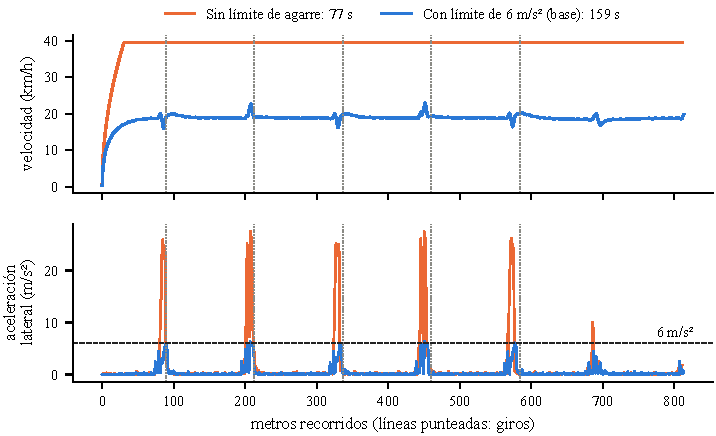
\includegraphics[width=0.68\linewidth]{figuras/fig_velocidad.pdf}
\caption{Velocidad y aceleración lateral a lo largo de una ruta del centro, para la red sin límite de agarre y para la red base, con límite de 6\,m/s$^2$. Es la ruta de más giros, de las 20 fijas, a la que llegan las dos.}
\label{fig:velocidad}
\end{figure}

% ---------------------------------------------------------------------
\subsection{Comparación de operadores genéticos}

Las cinco primeras filas de la Tabla~\ref{tab:redes} comparan los operadores, todos con límite de agarre.
En el centro llegan en 15 a 20 de las 20 rutas, y los intervalos de confianza se superponen.
Con 20 rutas y una sola semilla, ninguna diferencia se puede atribuir al operador.
El cruce por neurona, por ejemplo, fue el que menos llegó, pero su intervalo se superpone con los de todos los demás.
Montana y Davis tampoco encontraron diferencias claras entre sus tipos de cruce \cite[p.~766]{montana1989}\footnote{«Indican que hay poca diferencia de rendimiento entre los distintos tipos de cruce».}.
Todos los operadores, entonces, permiten aprender la tarea.

La Figura~\ref{fig:entrenamiento} muestra cómo aprende cada red.
Todas aprenden la manzana en 48 a 70 generaciones y pasan el 2$\times$2 en 10 a 25.
En la manzana, todas pasan primero por la mitad de las vueltas de referencia: aprenden a doblar hacia un lado antes que hacia el otro.
Al pasar al 2$\times$2 y al 3$\times$3, la mejor red ya llega en la mayoría de las rutas desde las primeras generaciones.
La red sin límite de agarre aprende más rápido, porque puede doblar a cualquier velocidad.

\begin{figure}[!htb]
\centering
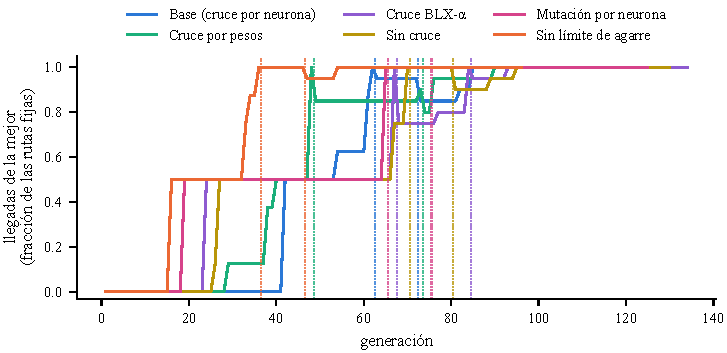
\includegraphics[width=0.68\linewidth]{figuras/fig_entrenamiento.pdf}
\caption{Llegadas de la mejor red guardada en las rutas de referencia de su etapa, generación por generación: 8 vueltas en la manzana y 20 rutas en el 2$\times$2 y en el 3$\times$3. Las líneas punteadas verticales marcan, con el color de cada red, el paso a la etapa siguiente.}
\label{fig:entrenamiento}
\end{figure}

% ---------------------------------------------------------------------
\subsection{Generalización a calles nuevas}

El centro contiene a los recortes de entrenamiento, que son cerca del 22\,\% de su calzada.
Pero suma diagonales, una avenida curva y un cruce de siete calles que no aparecen en ellos.
Aun así, las seis redes llegan en 15 a 20 de sus 20 rutas (Tabla~\ref{tab:redes}).
El cruce de siete calles es un error del mapa: quedó al unir en un nodo esquinas a menos de 10\,m.
Por él pasan 8 de las 20 rutas, y ahí ocurren 7 de las 10 fallas de las redes con límite.

Para probar en calles que nunca vieron, cada red manejó además las 20 rutas fijas de un barrio de prueba (Tabla~\ref{tab:barrios}).
Todas manejan en esos barrios, con entre 7 y 20 llegadas.
Cada red se probó en un barrio distinto, así que esta tabla no compara operadores: para eso está la del centro.
Lo que muestra es que redes entrenadas en una manzana y dos recortes chicos manejan en barrios nuevos.
Una explicación es que sus sensores miden todo desde el auto, y así una esquina se ve parecida en cualquier mapa.

\begin{table}[!htb]
\centering
\caption{Cada red en las 20 rutas fijas de un barrio de prueba. Entre corchetes, el intervalo de confianza del 95\,\% de la tasa de llegada.}
\label{tab:barrios}
\small
\begin{tabular}{llccc}
\toprule
Red & Barrio & Llegadas & Choques & Sin tiempo \\
\midrule
Base: cruce por neurona & Guadalupe & 10 / 20 \; [27--73\,\%] & 10 & 0 \\
Cruce por pesos & Roma & 19 / 20 \; [75--100\,\%] & 1 & 0 \\
Cruce BLX-$\alpha$ & Schneider & 12 / 20 \; [36--81\,\%] & 6 & 2 \\
Sin cruce & 12 de Octubre & 20 / 20 \; [83--100\,\%] & 0 & 0 \\
Mutación por neurona & La Guardia & 7 / 20 \; [15--59\,\%] & 11 & 2 \\
Sin límite de agarre & Arenales & 13 / 20 \; [41--85\,\%] & 7 & 0 \\
\bottomrule
\end{tabular}
\end{table}

% =====================================================================
\section{Conclusiones}
\label{sec:conclusiones}

En este trabajo, un algoritmo genético entrenó un perceptrón multicapa de 306 pesos que maneja por calles reales de Santa Fe.
El aporte fue juntar piezas de trabajos anteriores en mapas reales y agregar un límite de agarre al modelo del vehículo.
Con una sola semilla, las diferencias entre operadores no alcanzaron para ordenarlos, y todos resultaron capaces de aprender la tarea.
El límite de agarre resultó necesario: sin él, la red aprovecha una física imposible, y con él maneja dentro de lo que un auto real puede hacer.
La red aprende lo que la física y la aptitud le piden, y eso permite guiar su comportamiento.

Como trabajos futuros quedan usar varias semillas y probar todas las redes en los mismos barrios.
También se puede sumar el premio por tiempo, para buscar redes que frenen antes de las esquinas.
Otra línea es comparar el entrenamiento directo con el entrenamiento por etapas.
Por último, el tráfico y los semáforos exigirían nuevos sensores y otra aptitud.

% =====================================================================
{\small
\setlength{\bibsep}{1pt}
\bibliographystyle{unsrtnat}
\bibliography{refs}}

% Las citas textuales, en una hoja aparte después de las referencias
\newpage
\theendnotes

\end{document}
